% Paper 1 --- Patterns active manuscript, v30t (2026-10-22).
% Title: Annotation accuracy is not a proxy for differentiation order in
%        fine-tuned single-cell foundation models.
% Build: pdflatex -> bibtex -> pdflatex x2, output to latex/build/.
% Bibliography: paper1.bib (88 entries).
% State: figure-audit pass --- Figure 2 caption names the L9 seed rebound,
%        Figure 4 retitled to what its panels show (gradient claim moved to
%        Figure 2), Figure 1(B) arm list and Figure 6(C) layout wording
%        brought in line with the redrawn panels. No numbers changed.
\documentclass[12pt,letterpaper]{article}
\usepackage[a4paper, total={7in, 10in}]{geometry}
\renewcommand{\familydefault}{\sfdefault}
\usepackage{graphicx}
\usepackage{helvet}
\usepackage{authblk}
\usepackage[hidelinks]{hyperref}
\usepackage{amsmath}
\usepackage{amssymb}
\usepackage{orcidlink}
\usepackage[super,comma,sort&compress]{natbib}
\bibliographystyle{numbered}
\usepackage[right]{lineno}
\linenumbers

\usepackage[utf8]{inputenc}
\usepackage[T1]{fontenc}
\usepackage{booktabs}
\usepackage{microtype}
\emergencystretch=3em
\usepackage{tabularx}
\usepackage{array}
\usepackage{ragged2e}

\makeatletter
\renewcommand{\maketitle}{\bgroup\setlength{\parindent}{0pt}
\begin{flushleft}
  \textbf{\@title}

  \@author
\end{flushleft}\egroup}
\makeatother

\title{Annotation accuracy is not a proxy for differentiation order in fine-tuned single-cell foundation models}
\date{}

\author[1,2]{Kunhui Xu~\orcidlink{0009-0001-5881-9858}}
\author[1]{Chenchen Wang~\orcidlink{0009-0004-7200-5190}}
\author[1]{Fenfen Li~\orcidlink{0000-0001-5577-4562}}
\author[2]{Xiaoyu Chen~\orcidlink{0000-0002-9980-5524}}
\author[2]{Xinyu Wang~\orcidlink{0009-0006-1182-8964}}
\author[2]{Yi Zhang~\orcidlink{0009-0001-7220-1229}}
\author[2]{Tiancheng Pu~\orcidlink{0009-0005-2117-6317}}
\author[2]{Jiahao Tang~\orcidlink{0009-0001-1648-8480}}
\author[1,*]{Hongguang Cui~\orcidlink{0000-0001-7311-0188}}
\author[2,*]{Peng Guo~\orcidlink{0009-0004-8215-7673}}
\author[1,2,*,\dag]{Qi Dai~\orcidlink{0000-0002-9950-6161}}

\affil[1]{The First Affiliated Hospital, Zhejiang University School of Medicine, 1367 Wenyi West Road, Yuhang District, Hangzhou, Zhejiang Province 311121, PR China}
\affil[2]{Eye Research Center, Hangzhou Institute of Medicine, Chinese Academy of Sciences, Eye Hospital, Wenzhou Medical University, Hangzhou, Zhejiang Province 310018, PR China}
\affil[*]{Correspondence: Hongguang Cui (\nolinkurl{1189002@zju.edu.cn}), Peng Guo (\nolinkurl{guopeng@ucas.ac.cn}), and Qi Dai (\nolinkurl{dq@mail.eye.ac.cn}).}
\affil[{}\dag]{Lead contact.}

\begin{document}

\maketitle

\section*{Summary}

Fine-tuning a single-cell foundation model is usually judged by how well it labels held-out cells, not by whether its embedding still orders those cells along a developmental sequence. We measured both in corneal epithelium before and after fine-tuning, across Geneformer, scGPT-human and CellPLM, with donor-disjoint splits and repeated training. In Geneformer, macro-F1 rose from 0.4421 to 0.6492 while the ordering correlation fell from 0.8064 to -0.0082. A cross-entropy head given the same four stage labels retained only 0.254, whereas an ordinal head held 0.833. The loss was conditional: it shrank out of corpus, reversed in two epidermal controls, and depended on architecture and training length. Ordinal supervision held across in-corpus settings but fell below cross-entropy on a post-cutoff test (three-seed means). We provide the evaluation as a reusable benchmark.

\section*{Keywords}

single-cell foundation models, classification fine-tuning, differentiation gradient, ordinal regression, contamination-aware benchmark, corneal epithelium, parameter-efficient adaptation, cross-architecture evaluation

\section*{Introduction}

Geneformer and scGPT learn representations from large single-cell corpora for cell-type prediction and analyses of gene and cellular variation \cite{theodoris2023,chen2026natcompsci,cui2024scgpt}, and fine-tuning optimizes these representations for classification on annotated datasets. Their subsequent use in differentiation analysis depends on whether the adapted embeddings retain the ordering of successive states, not only the separation of labeled populations. Here, we examine differentiation geometry before and after classification fine-tuning.

Benchmarks of annotation report consistent gains from adaptation: BioLLM measures improved precision and macro-F1 after fine-tuning scGPT and Geneformer \cite{qiu2025biollm}, although foundation models do not outperform task-specific methods across eight tasks \cite{liu2026} or in a thirteen-model deployment comparison \cite{hou2026}. These studies hold the prediction task fixed and vary the supervision regime. Parameter-efficient updates recover populations that full fine-tuning misclassifies \cite{he2026scpeft}, and downstream scores prove insensitive to pretraining scale \cite{finetuningmasking2026}, but none of these readouts measures whether the continuous ordering of states survives adaptation.

Order has been measured in frozen representations and in adjacent tasks. UCE organizes cells by developmental lineage and stage without task-specific fine-tuning \cite{rosen2026uce}. A zero-shot dynamics benchmark found stronger reconstruction with HVG/PCA and identified temporal compression and branch linearization in frozen foundation-model embeddings \cite{zhou2026}. EMP-FM reports that naive fine-tuning struggles to distinguish epithelial--mesenchymal intermediate states and adds pseudotime regression to resolve them \cite{pan2024}. Layerwise analyses map biological signals across network depth \cite{kendiukhov2026genomics,kendiukhov2026bioinformatics}, and circuit-level steering in a frozen Geneformer reports layer-dependent control of maturation, with the latest layers pushing cells toward maturity and earlier layers away from it \cite{kendiukhov2026circuits}. Ontology-informed evaluation scores frozen embeddings against known cell-type relationships \cite{wu2025}, and hierarchical cross-entropy encodes subtype relationships in the training target \cite{hce2026}. Each addresses a different object --- a frozen embedding, a supervised auxiliary task, or a label hierarchy --- and none pairs a frozen and an adapted representation to ask whether the same continuous order remains readable.

Corneal epithelial renewal links limbal stem and progenitor populations, proliferative intermediates, basal epithelial cells, and differentiated surface cells, and single-cell atlases characterize their molecular identities and spatial localization. Stem and early progenitor cells divide infrequently, whereas transiently amplifying populations show active proliferation \cite{collin2021,ligocki2021,li2021oculsurf}. Progenitor populations occupy the limbal niche, proliferative cells contribute to basal renewal, and differentiated populations form the superficial epithelium. We define the differentiation gradient as the association between a representation-derived cell ordering and a biologically specified stage order. We examine stemness, proliferation, and differentiation expression programs along this gradient to determine which aspects of the annotated renewal sequence remain represented after fine-tuning.

Classification gains coexist with loss of the differentiation gradient in Geneformer on the same-corpus corneal holdout, whereas an ordinal head preserves the gradient at comparable classification performance. Our predictability--computability--stability (PCS)-guided evaluation combines donor-disjoint comparisons and tests across pretraining-corpus boundaries with repeated training and perturbations of the differentiation-axis measurement \cite{ness2026}. We extend the frozen-versus-adapted comparison to scGPT-human and CellPLM, using an out-of-corpus corneal test and epidermal controls, and layer-resolved analyses locate the changes within each model. Combining the ordinal head with low-rank adaptation improves gradient retention and classification performance on the scGPT-human same-corpus test. The separate Geneformer ordinal head recipe loses its advantage on the post-cutoff test, and sensitivity to training seeds and checkpoint selection differs across models.

\section*{Results}

\subsection*{Geneformer fine-tuning improves annotation but collapses the differentiation gradient on the same-corpus holdout}

Geneformer classification fine-tuning improved annotation on GSE153515, while its differentiation gradient fell to near zero over the same runs. We evaluated 14,775 epithelial cells from two donors held out from supervised training, and the source study was represented in the pretraining corpus. We compared naive cross-entropy (CE) fine-tuning with frozen Geneformer-V2-104M plus a linear probe and HVG/PCA plus a linear classifier. The differentiation gradient was measured as Spearman correlation between representation-derived cell ordering and prespecified stage ranks, where cell ordering used projection onto the leading stage-centroid axis, oriented from limbal stem cells to differentiated cells. Layer adjacency accuracy (LAA) assessed local stage adjacency (Methods). Reference arms were single runs, and adapted-arm summaries below are means across three seeds (Figure~\ref{fig:pipeline}).

Fine-tuning increased donor-level macro-F1 from 0.4421 for the frozen Geneformer to 0.6492, while over the same cells the differentiation-gradient correlation fell from 0.8064 to -0.0082. A paired donor-stratified cell bootstrap placed this shift at 0.815 (95\% CI 0.692--0.908) with no replicate at or below zero, and per-seed shifts ranged from 0.752 to 0.849 and shared the same direction in both test donors (Figure S3). LAA, a low-sensitivity companion metric, rose by only 0.010 over the same runs (0.9665 to 0.9768; 95\% CI 0.007--0.013), against the 0.32 and 0.33 by which the frozen and naive arms exceeded the label-permutation null mean for this metric (0.642), so layer adjacency does not track the loss of stage order (Table~\ref{tab:external}; Figure~\ref{fig:external}). Both test donors showed higher macro-F1 than the frozen Geneformer in all three adapted runs. The naive runs also failed to recover the rare TAC class (171 cells; 1.2\%), and per-class results and the three-class sensitivity analysis are provided in the Supplementary Information (Figure S9).

The HVG/PCA reference retained a differentiation-gradient correlation of 0.8206 and achieved macro-F1 of 0.6192, with a local layer adjacency that was also high (LAA 0.9771). Naive fine-tuning therefore had a numerically higher macro-F1 than this reference but a much weaker gradient, and HVG/PCA and the frozen Geneformer representation both retained strong stage-order associations (Table~\ref{tab:external}). Frozen probes for scFoundation and UCE are reported in Table S4; they did not enter the paired adapted comparison.

Our layer-resolved measurements placed the largest loss in the upper part of Geneformer (Figure~\ref{fig:layerwise}). Across the frozen and naive representations, L1--L4 correlations ranged from approximately 0.41 to 0.84, and at L3 the adapted correlations were 0.81--0.84 compared with 0.766 in the frozen model. The adapted profiles declined in the upper layers, with seed-dependent rebounds, including a pronounced L9 rebound in seed 123. At L12, the frozen representation reached its strongest gradient, whereas the adapted checkpoints ended near zero, with their reported cell-level bootstrap 95\% confidence intervals each spanning zero. The early-layer signal thus remained accessible after the final-layer loss.

\subsection*{Adaptation flattens the stemness gradient and weakens the corneal differentiation signal}

On the same GSE153515 cells, naive fine-tuning weakened the association of corneal expression programs with representation-derived pseudotime. To relate this loss to corneal progenitor and differentiated states \cite{collin2021,ligocki2021}, we correlated fixed expression-program scores with each model's axis pseudotime, and scores were means of z-scored log1p expression, unchanged across models. For frozen Geneformer, stemness declined along the axis (Spearman correlation -0.407; cell-bootstrap 95\% CI -0.421 to -0.394), while the KRT12/KRT3 differentiation program increased (+0.69; 95\% CI +0.68 to +0.70). Across three naive runs, stemness correlation was +0.02 $\pm$ 0.03 and differentiation correlation +0.29 $\pm$ 0.03 (mean $\pm$ population SD across seeds; ddof = 0), and representative single-run axis profiles are shown in Figure~\ref{fig:bio}B.

The gene-level changes included KRT15, whose correlation shifted from -0.53 in frozen embeddings to -0.06 in the naive seed-42 run. KRT19 shifted from -0.41 to -0.12 in the same comparison. Some program genes overlap the annotation marker sets (Methods), and NFIB and CDH3 were not used for annotation but contributed to the stemness score, with separate frozen-axis correlations of -0.16 and -0.07. TP63 behaved differently: it was basal-peaked, not stem-cell-peaked, in this dataset, with a weak positive frozen-axis correlation (+0.13) instead of the declining stemness-program association.

Cycling expression distinguished the proliferative TAC compartment from the low-cycling compartments, consistent with the biological distinction between slow-cycling limbal cells and proliferative progeny \cite{cotsarelis1989}. Mean cycling score was 3.15 in TAC cells versus less than 0.05 in each other corneal class (Figure~\ref{fig:bio}D, corneal bars), and PCNA and MCM2, absent from the annotation marker sets, also peaked in TAC. This TAC-enriched cycling pattern reflects fixed expression differences between compartments, not preservation of an axis-dependent gradient after adaptation.

\subsection*{The gradient loss shrinks out of corpus and reverses in epidermis}

The severe Geneformer loss on GSE153515 did not extend uniformly to other evaluation domains. We compared that same-corpus holdout (the same tissue as the training atlas, represented in the pretraining corpus) with GSE299152, a post-cutoff out-of-corpus ocular-surface dataset \cite{gse299152}, and human epidermis as a cross-tissue control (a different tissue from the same corpus). GSE299152 contributed 21,374 epithelial cells from three donors and was deposited after assembly of Genecorpus-104M, with no matching source DOI in its table, and its frozen gradient correlation was 0.707 compared with 0.641 $\pm$ 0.030 after naive fine-tuning (three-seed mean $\pm$ SD). The adapted runs retained a positive stage-order association, unlike the near-zero GSE153515 endpoints (Table~\ref{tab:domains}; Figure~\ref{fig:domains}). On GSE147424 epidermis \cite{he2020epidermis}, the direction reversed: the single seed-42 Geneformer checkpoint increased correlation from 0.239 to 0.455, and a second epidermal dataset, GSE202352 \cite{wiedemann2023}, gave 0.518 frozen and 0.714 after naive fine-tuning, also from seed 42. Both epidermal sources were represented in the pretraining corpus, separating corpus membership from the direction in which the change went.

The epidermal program readouts also differed from the corneal result. On GSE147424, the basal-keratin program comprising KRT5, KRT14, and COL17A1 declined along the frozen axis and more strongly along the naive axis (correlations -0.59 and -0.75), and the naive cycling-program correlation was -0.23. This basal-off component accords with the basal-to-suprabasal keratin transition \cite{fuchs1980}, whereas the differentiation-pole keratins were less uniformly ordered, with KRT1 reported as bimodal and KRT10 correlation only +0.18 in the ordinal example. On GSE202352, the frozen representation carried a differentiation-pole signal but little basal-off association (basal-program correlation +0.11). Adapted axes recovered negative basal-program associations across the evaluated recipes (-0.65 to -0.79), and the naive cycling association was -0.21 (Figure~\ref{fig:bio}C). The two frozen representations emphasized different parts of the epithelial program rather than recovering an identical biological ordering.

Under Geneformer's official one-epoch budget, the six runs with seeds 42, 123, 456, 789, 2024, and 31415 had gradient correlations ranging from -0.133 to 0.201 (mean 0.058; per-seed values in Table S8). The first three seeds alone gave mean 0.096, and the six-seed summary is distinct from that earlier subset, with both summaries well below the frozen reference. The main three-epoch protocol ended at mean -0.008, so the loss was already present under the shorter evaluated budget and was not confined to the three-epoch endpoint. The per-seed budget comparison remains in the Supplementary Information.

We ran two further scGPT corneal evaluations that illustrated the role of the data context. On GSE186433, frozen correlation was 0.4180 and the best-validation naive checkpoints reached 0.8158 and 0.8192 for seeds 42 and 123, with macro-F1 0.8868 and 0.8481. On GSE155683, frozen correlation was 0.5285 and the corresponding adapted values were 0.8362 and 0.8775, with macro-F1 0.9546 and 0.9495, and both datasets were absent from the reported pretraining census. The scGPT epidermal control did not show uniform rebuilding: its best-validation and final-epoch outcomes varied across seeds, including a negative best-validation correlation in one run. Across these evaluations, stronger frozen axes often accompanied larger losses, but neither source inclusion nor initial axis strength supplied a sufficient rule for predicting the outcome.

\subsection*{Loss depth and seed sensitivity differ across architectures}

For cross-model comparisons, we constructed a separate same-corpus arm using the van Zyl corneal atlas \cite{vanzyl2022}, represented in scGPT-human's pretraining census \cite{cui2024scgpt}. We excluded the ciliary-muscle cluster, leaving 62,640 epithelial cells in this arm, and held out donor Hu0216 (20,158 epithelial cells) for testing. Unlike the four-stage Geneformer evaluation, the locked van Zyl axis had three stages, LSC to basal to differentiated: the gene filter removed the cycling markers needed to resolve a separate TAC class. Its frozen test-donor correlation was 0.789, and the scGPT readout used L2-normalized embeddings. These dataset, stage-resolution, and readout differences make the comparison a test across model configurations, not an intervention on architecture alone (Figure~\ref{fig:spectrum}).

scGPT-human showed stronger checkpoint and seed dependence. After a 15-epoch training schedule, the checkpoints selected by validation macro-F1 had test-donor correlations of 0.337, 0.577, and 0.404 across seeds 42, 123, and 456 (mean 0.440), with mean macro-F1 0.931. Validation-gradient peaks occurred at epochs 3, 3, and 6, whereas checkpoints were selected by validation macro-F1, and test-donor gradient scores were not used for selection. Final-epoch evaluation additionally included seeds 789 and 2024, and across those five seeds correlations ranged from -0.091 to 0.833 (per-seed values in Table S7). Some final checkpoints retained the gradient, whereas seed 42 lost it. The best-validation comparison used three seeds, and the final-epoch sensitivity analysis used five.

The endpoint was also sensitive to head initialization within the scGPT configuration. With the remaining protocol fixed, head scales 0.01 and 1.0 and head seed 999 produced final correlations of 0.572, 0.786, and 0.804, against -0.091 for the default seed-42 run.

CellPLM provided a third model configuration on the same van Zyl test donor, for which the seed-42 frozen reference gave correlation 0.865. Naive cross-entropy fine-tuning at the convergence budget gave a three-seed mean of -0.007 $\pm$ 0.035 (sample SD), and the next section shows that this endpoint depends on training length. In the seed-42 layerwise analysis, correlation fell from 0.906 at the embedder output to 0.118 at L1, whereas frozen L1 remained at 0.771, an early drop that differed from Geneformer's upper-layer pattern. Separate two-seed CellPLM consistency tests increased the epidermal correlation from a frozen reference of 0.094 to 0.835 $\pm$ 0.006, but decreased the leave-one-donor Hu0220 corneal correlation from 0.814 to 0.659 $\pm$ 0.008. These separate tissue and donor protocols retained positive correlations, unlike the near-zero Hu0216 endpoint.

\subsection*{In CellPLM the mean gradient loss emerges after accuracy plateaus}

The CellPLM endpoint depended on training length. At the three-epoch budget of the Geneformer comparison, naive cross-entropy retained the gradient (three-seed mean 0.879 $\pm$ 0.012). Fifteen epochs gave 0.862 $\pm$ 0.044 at macro-F1 0.959. Thirty epochs gave 0.779 $\pm$ 0.095 at macro-F1 0.971, and sixty epochs gave 0.122 $\pm$ 0.291, with individual seeds spanning $+0.457$ to $-0.062$. The convergence runs (83, 97 and 118 epochs) ended at $-0.007$ $\pm$ 0.035, while macro-F1 rose from 0.835 to 0.973 over the same range and changed little after 30 epochs. In this architecture the mean loss tracked optimization that continued after macro-F1 had plateaued, not the approach to plateau itself (Figure~\ref{fig:spectrum}C).

Ordinal supervision with low-rank adaptation retained the gradient at the convergence budget ($0.922 \pm 0.0003$ across three seeds, one of which continued to 454 epochs), at a macro-F1 of 0.950 against 0.973 for cross-entropy. Ordinal supervision alone reached $0.918 \pm 0.002$ at the same stage, so the adapters contributed little on this architecture (Table S11).

\subsection*{Ordinal supervision and LoRA preserve stage ordering in same-corpus tests}

An ordinal head retained the Geneformer gradient on the same-corpus holdout. The implemented head used unconditional cumulative-threshold binary cross-entropy over the known stage ranks, with a separate threshold output for each transition and threshold-count class decoding, and did not impose equal spacing between stages. On Geneformer, the ordinal loss was restricted to epithelial cells, whereas the original cross-entropy task used 31 author-assigned classes before harmonization to the four epithelial evaluation classes.

Under the three-epoch Geneformer protocol, the ordinal head achieved mean gradient correlation 0.833 across three seeds, with range 0.830--0.835, and donor-level macro-F1 0.649. Its observed macro-F1 was close to the naive result, and its gradient was substantially stronger. Giving cross-entropy the same four stage labels retained a correlation of 0.254 (three seeds, 7,473 steps). A matched arm restricted to the epithelial subset (2,616 steps) retained 0.158. The step-matched cross-entropy arm was 0.579 below the ordinal head (95\% CI 0.541 to 0.631 below). The ordinal + continuity arm gave correlation 0.828 (range 0.824--0.832) and macro-F1 0.648, with LAA approximately 0.97 in both ordinal arms (Table~\ref{tab:external}), and its mean correlation was approximately 0.005 lower than the ordinal head result.

The ordinal Geneformer axes also retained the expression-program associations introduced above. The ordinal head stemness correlation averaged -0.427 across three seeds, compared with -0.407 in the frozen reference and near-zero association after naive adaptation. Its differentiation-program correlation averaged +0.557, below the frozen +0.690 but above the naive +0.286, and the ordinal + continuity stemness mean was -0.407. These correlations used the same fixed expression scores, with NFIB and CDH3 included in the stemness score.

The scGPT comparisons used two budget and checkpoint settings (Table S12). At three epochs with final-epoch evaluation, cross-entropy gave gradient correlation 0.5554 $\pm$ 0.2521 and macro-F1 0.9225 $\pm$ 0.0092, while the ordinal head gave 0.8188 $\pm$ 0.1487 and 0.9587 $\pm$ 0.0080, respectively (three-seed means $\pm$ sample SD). The ordinal correlations ranged from 0.647 to 0.907, showing seed variation under this shorter protocol.

For the 15-epoch best-validation comparison, we evaluated cross-entropy, LoRA-only, and ordinal + LoRA using seeds 42, 123, and 456. LoRA introduced low-rank updates to the attention query/key/value projections (rank 8, scaling factor 16), and each arm used 38,235 training cells and 4,247 validation cells, with checkpoint selection by validation macro-F1. Cross-entropy achieved mean correlation 0.4395 $\pm$ 0.1240 and macro-F1 0.9311 $\pm$ 0.0109, LoRA-only gave 0.8665 $\pm$ 0.0253 and 0.9342 $\pm$ 0.0044, and ordinal + LoRA gave 0.9241 $\pm$ 0.0006 and 0.9659 $\pm$ 0.0024 (sample SD). The combined recipe had the highest observed correlation and macro-F1 among these matched adapted arms, whereas the ordinal head runs used a different training partition, three epochs, and final checkpoints.

Final checkpoints retained a similar pattern within the parameter-efficient recipes. LoRA-only gave mean correlation 0.8436 and macro-F1 0.9435, while ordinal + LoRA gave 0.9226 and 0.9635 across the same three seeds. The frozen gradient reference was 0.789, and frozen macro-F1 was 0.969 in a within-test-donor self-probe.

CellPLM's ordinal arm also retained stage ordering on Hu0216 (three-seed correlation 0.918 $\pm$ 0.002; cross-entropy -0.007 $\pm$ 0.035; sample SD). Both three-seed mean macro-F1 values rounded to 0.9728, with sample SD 0.0003 for cross-entropy and 0.0013 for the ordinal arm. Its separate single-seed LoRA run achieved correlation 0.873 and macro-F1 0.958, and that run did not include an ordinal head. On the post-cutoff Geneformer test, the ordinal head arm gave correlation 0.350 $\pm$ 0.099 and the ordinal + continuity arm 0.539 $\pm$ 0.007, both below cross-entropy's 0.641 $\pm$ 0.030 (three-seed means; no paired bootstrap was computed for this domain). Their macro-F1 means were approximately 0.29--0.30, compared with 0.452 for cross-entropy. The combined ordinal + LoRA strategy was evaluated only on the same-corpus scGPT test.

We asked, in a parallel comparison on the same locked test donor, whether the frozen foundation-model representation is itself the strongest available description of this axis. Six classical baselines --- harmony, four HVG/PCA variants, and scVI --- reached gradient correlations of 0.840 to 0.865, all above the frozen scGPT-human reference (0.789) and far above naive cross-entropy fine-tuning (0.440), with scVI highest at 0.865. The ordinal + LoRA recipe (0.924) remained above every baseline, but its margin over the strongest classical baseline, 0.059, is smaller than the gap that fine-tuning opens between the frozen and naive arms. This benchmark therefore measures the readability of an existing differentiation gradient, and it does not establish that foundation-model representations outperform classical ones on this axis (Table S10).

\subsection*{Controls reproduce the loss and separate the readout from the axis choice}

We also ran diffusion pseudotime (DPT), which recovered weaker stage ordering from adapted Geneformer embeddings. Rooted in the LSC class on the same external cells, it correlated with the reference stage ordering at 0.850 for frozen embeddings (95\% CI 0.842--0.858), compared with 0.323--0.348 for the naive checkpoints (Figures S11 and S13). In the locked-axis diagnostic, frozen stage-centroid projections were ordered with centroid-level Spearman correlation 1.0, whereas the naive seed-42 centroids gave 0.4, and the frozen stage-centroid axis was not identical to the dominant per-cell variance direction (cosine 0.412).

CellPLM sensitivity results depended on the axis definition: the first stage-centroid component reproduced the collapse-and-retention criteria in all three seeds, with verdict ROBUST. The second centroid component and second and third per-cell principal components were all labeled PARTIAL: ordinal retention met the criterion, but naive collapse did not. With the second centroid component, the frozen correlation was approximately 0.260 and the naive correlations approximately 0.914--0.917.

Marker and rank perturbations showed a similar distinction. For the locked van Zyl, canonical-mini, and data-derived marker panels, all three CellPLM seeds received ROBUST verdicts for the centroid-marker readout, whereas marker-axis alignments were less consistent, with PARTIAL verdicts in the locked and canonical panels and in the data-derived seed-42 run. Shifting the ordinal ranks or changing their spacing while preserving their order retained ROBUST verdicts, as expected for a rank statistic. Reversing the ranks changed the sign and produced PARTIAL verdicts under the directional criteria, and the non-monotone reassignment gave one ROBUST and two PARTIAL verdicts.

In a separate fixed-frozen-axis control, we examined whether the projection was refitted for each checkpoint. On the scGPT Hu0216 test donor, a direction was fitted once from reference-labeled frozen stage centroids and then reused on adapted embeddings. The frozen self-projection gave correlation 0.7887, and ordinal + LoRA retained a three-seed mean correlation of 0.9215 under that fixed direction, compared with 0.9241 under checkpoint-specific axes. The three-epoch naive checkpoints gave mean 0.6561 under the fixed direction, and individual values were 0.6887, 0.5668, and 0.7126. The projection improved the readout for some naive checkpoints and weakened it for others relative to their individually fitted axes, while ordinal head checkpoints ranged from 0.7469 to 0.9169 under the fixed direction.

In the primary 26-test multiplicity family, the frozen and ordinal gradient correlations had adjusted q values approximately 0.009, and the naive positive-correlation test had q = 1.0. These q values test positive association, and the contrast between frozen and adapted arms is quantified separately by a paired bootstrap (Methods). A separate cross-model family contained 21 association tests, with 20 positive associations significant at q < 0.05, while the later-completed CellPLM cross-entropy and ordinal tests and the scGPT ordinal + LoRA test were outside that family. Across these controls, the ordinal arms retained the gradient and the cross-entropy arms did not. Nevertheless, how large the cross-entropy loss was depended on the axis definition, and two axis variants returned only partial collapse verdicts.

% ---- floats in original source order; Figure 3/table text updated ----
\begin{figure}[htbp]
\centering
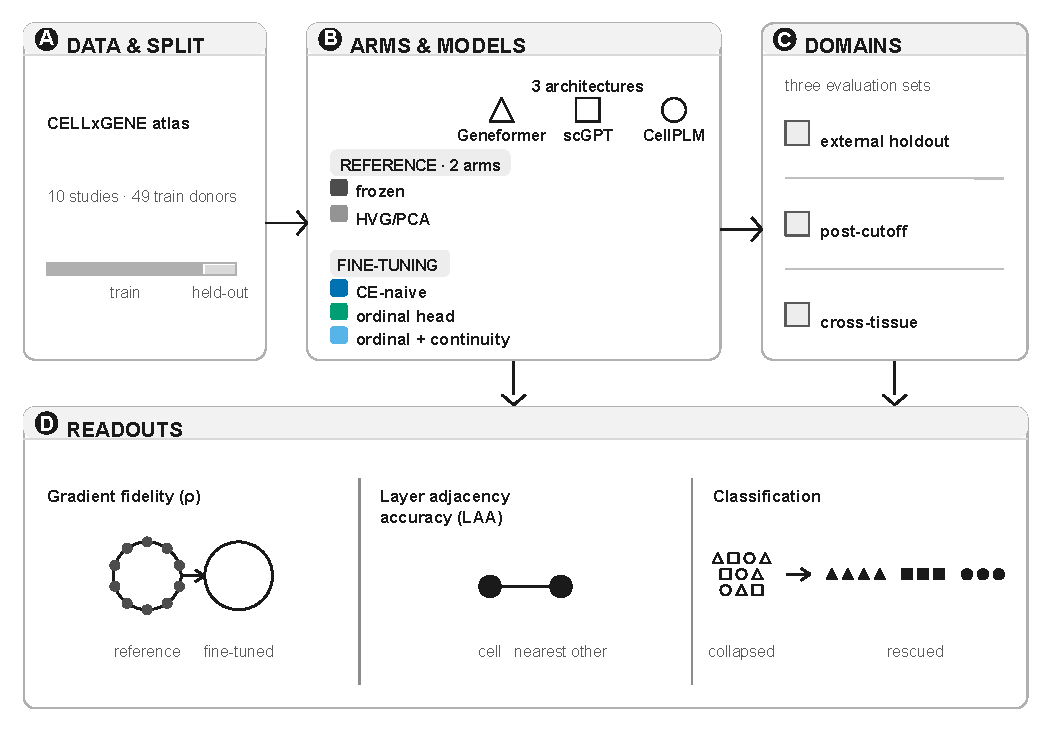
\includegraphics[width=1.0\textwidth]{../../../../figures/paper1/figure1_pipeline_overview}
\caption{Study pipeline (schematic readouts, not measured performance). (A) Data \& split: the donor-disjoint CELLxGENE training atlas and the train/held-out split. (B) Arms and models: reference arms (frozen, HVG/PCA) and the fine-tuning recipes that carry the main comparison (CE-naive, ordinal head, ordinal + continuity), across the three model families; LoRA and ordinal + LoRA are evaluated only in Figure~\ref{fig:spectrum}. (C) Domains: the in-corpus external holdout (GSE153515), post-cutoff out-of-corpus external test (GSE299152) and cross-tissue epidermis; coverage varies by model and domain. (D) Readouts: gradient fidelity ($\rho$); layer adjacency accuracy (LAA), the fraction of cells whose nearest other cell in Euclidean space has an identical or adjacent stage; and classification (macro-F1).}\label{fig:pipeline}
\end{figure}

\begin{figure}[htbp]
\centering
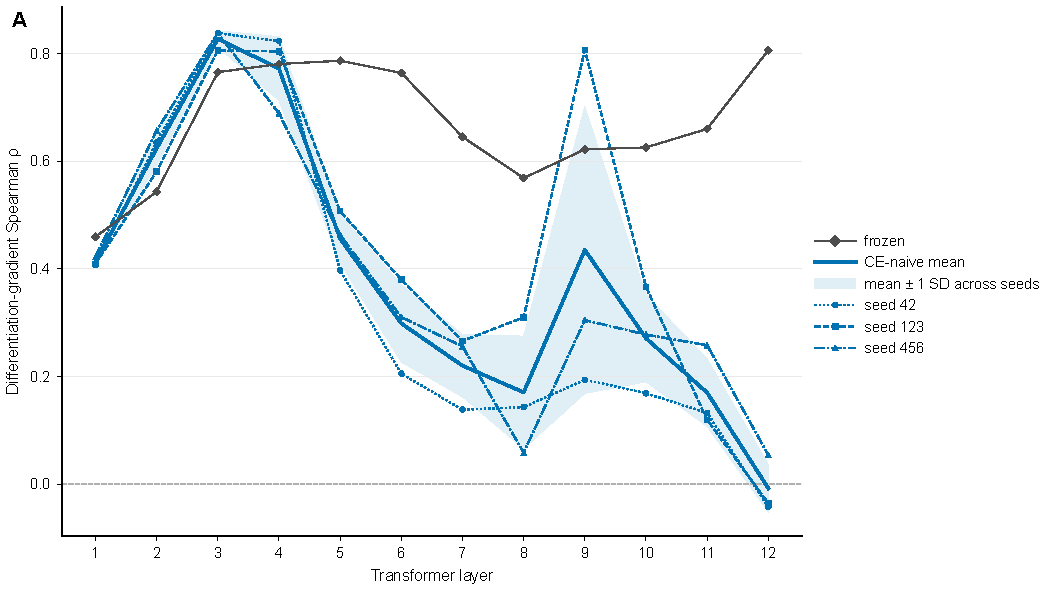
\includegraphics[width=1.0\textwidth]{../../../../figures/paper1/figure2_layerwise_rho}
\caption{Layer-resolved analysis localizes the collapse to upper transformer layers. Differentiation-gradient Spearman $\rho$ (y-axis) across hidden states L1--L12 (x-axis) for the Geneformer-based configurations (n = 14{,}775 in-corpus external holdout epithelial cells; three seeds per adapted arm). Color key: thick dark gray line, frozen Geneformer; blue line, CE-naive (seed mean over seeds 42, 123 and 456; n = 3, ddof = 0; shaded band = mean $\pm$ 1 population SD across seeds), with the individual seeds as thin lines. The gradient collapse under classification fine-tuning is head-proximal: early layers retain the gradient, while L5--L12 decay apart from a seed-driven rebound at L9. See also Figure S7 and Table S3.}\label{fig:layerwise}
\end{figure}

\begin{figure}[htbp]
\centering
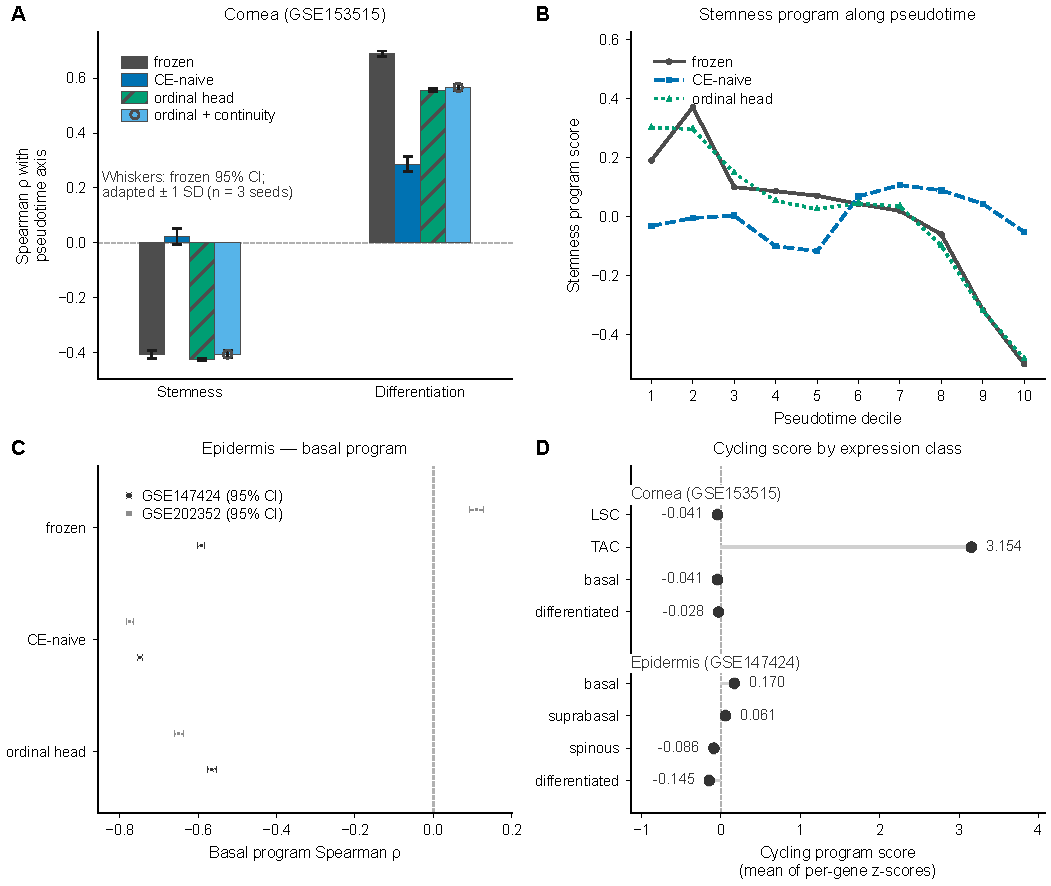
\includegraphics[width=1.0\textwidth]{../../../../figures/paper1/figure3_biological_readouts}

\caption{Gene-program readouts across representations and expression classes. (A) Spearman $\rho$ between fixed gene-program scores and each representation's pseudotime axis in cornea (GSE153515; 14,775 cells). Stemness: TP63, KRT15, KRT19, NFIB, CDH3; differentiation: KRT12, KRT3. Adapted bars: means over seeds 42, 123, 456, $\pm$1 population SD (ddof = 0); frozen: single reference, 95\% cell-bootstrap interval. (B) Cornea stemness score along pseudotime deciles, one checkpoint per arm, no intervals. (C) Basal-program $\rho$ (KRT5, KRT14, COL17A1) in epidermis, GSE147424 (18,355 cells) and GSE202352 (14,461 cells); points are single seed-42 checkpoints, 95\% cell-bootstrap intervals. Arms: panel A shows frozen, CE-naive, ordinal head and ordinal + continuity (open marker); panels B--D show frozen, CE-naive and ordinal head. (D) Cycling program score by expression class, fixed class means without intervals; cornea PCNA, MCM2, MKI67, TOP2A, epidermis MKI67, PCNA.}\label{fig:bio}
\end{figure}

\begin{figure}[htbp]
\centering
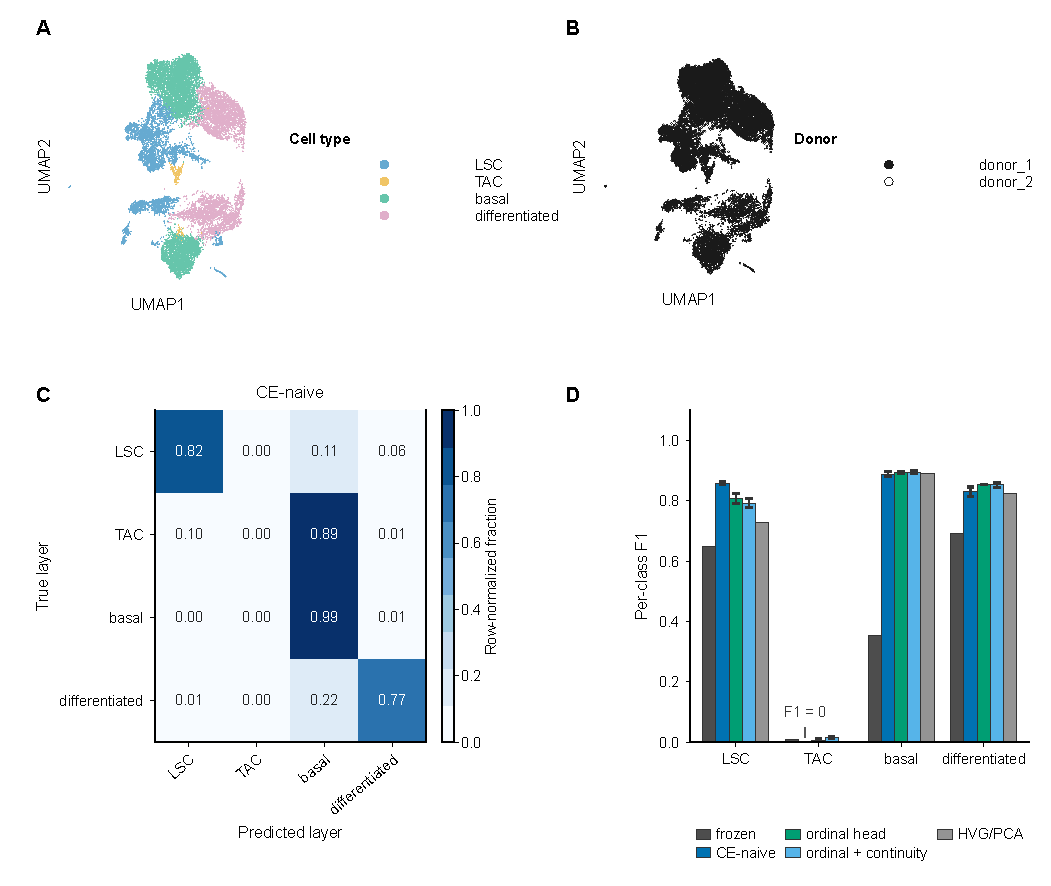
\includegraphics[width=1.0\textwidth]{../../../../figures/paper1/figure4_external_eval}
\caption{Same-corpus holdout: fine-tuning raises per-class F1 and annotation accuracy. Adapted models evaluated on GSE153515 (n = 14{,}775 epithelial cells, two donors); the differentiation-gradient collapse measured over the same runs is shown in Figure~\ref{fig:layerwise}. (A) Cell-type labels (external test). (B) Donor UMAP; fill alone encodes donor (donor\_1 filled, donor\_2 open, single hue). (C) CE-naive confusion matrix, row-normalized. (D) Per-class F1 across five model arms (frozen, CE-naive, ordinal head, ordinal + continuity, HVG/PCA; adapted arms are three-seed means $\pm$ 1 sample SD, reference arms are single runs with no interval); the TAC column shows F1 = 0 (n = 171; three-class sensitivity in Figure S9). Class supports: 3,423 LSC, 171 TAC (1.2\%), 6,698 basal and 4,483 differentiated cells. See also Figure S6.}\label{fig:external}
\end{figure}

\begin{table}[htbp]
\centering
\small
\caption{External test performance by model arm (GSE153515, four classes; n = 14{,}775 epithelial cells from two donors). Adapted-arm values and CI limits are averaged across three seeds; intervals use donor-level bootstrap 95\% CIs. Reference arms are single runs (seed 42). LAA, layer adjacency accuracy; ECE, expected calibration error.}\label{tab:external}
\begin{tabularx}{\textwidth}{@{}l X c c c c@{}}
\toprule
Model arm & Macro-F1 & 95\% CI & LAA & $\rho$ & ECE \\
\midrule
HVG/PCA + linear & 0.6192 & [0.5747, 0.6637] & 0.9771 & 0.8206 & 0.0145 \\
Frozen Geneformer & 0.4421 & [0.3749, 0.5093] & 0.9665 & 0.8064 & 0.3010 \\
\addlinespace[4pt]
CE-naive, 31-class ($\lambda=0$) & 0.6492 & [0.6233, 0.6751] & 0.9768 & $-0.0082$ & 0.0575 \\
CE, 4-class epithelial (2{,}616 steps) & 0.6604 & [0.6335, 0.6873] & 0.9806 & $+$0.1582 & 0.0770 \\
CE, 4-class epithelial (7{,}473 steps) & 0.6576 & [0.6286, 0.6866] & 0.9794 & $+$0.2541 & 0.1048 \\
Ordinal head ($\lambda=0$) & 0.6490 & [0.6100, 0.6879] & 0.9739 & $+0.8330$ & 0.1251 \\
Ordinal + continuity ($\lambda=0.5$) & 0.6479 & [0.6099, 0.6860] & 0.9749 & $+0.8277$ & 0.0609 \\
\bottomrule
\end{tabularx}
\bigskip
\footnotesize
\textbf{Note.} Reference arms are single runs; adapted arms are three-seed means. Macro-F1 is donor-level macro-averaged F1; CI, bootstrap 95\% confidence interval; LAA, layer adjacency accuracy; ECE, expected calibration error; $\rho$, differentiation-gradient Spearman correlation. The two CE, 4-class epithelial rows supervise the same cells and labels and differ in the batched cells and, consequently, in the optimizer-step budget (2{,}616 versus 7{,}473 steps); read against the ordinal head row, they separate the step budget from the label set. Against the frozen reference, the 7{,}473-step row sat 0.552 lower (95\% CI 0.514 to 0.604).
\end{table}

\begin{table}[htbp]
\centering
\small
\caption{Differentiation-gradient Spearman $\rho$ across evaluation domains (Geneformer-V2-104M arms). Same-corpus adapted values are three-seed means (per-seed ranges in parentheses); out-of-corpus values are three-seed means $\pm$ SD; cross-tissue and frozen values are single runs. Ordinal head, ordinal loss alone; ordinal + continuity, ordinal head with the continuity term ($\lambda = 0.5$). Em dashes mark domains not evaluated; BH--FDR control applies to the same-corpus family.}\label{tab:domains}
\begin{tabularx}{\textwidth}{@{}l X X X X@{}}
\toprule
Domain & Frozen & CE-naive & Ordinal head ($\lambda = 0$) & Ordinal + continuity ($\lambda = 0.5$) \\
\midrule
Same-corpus (GSE153515) & 0.806 & $-0.008$ ($-0.042$ to $+0.054$) & $+0.833$ (0.830--0.835) & $+0.828$ (0.824--0.832) \\
Out-of-corpus (GSE299152) & 0.707 & 0.641 $\pm$ 0.030 & 0.350 $\pm$ 0.099 & 0.539 $\pm$ 0.007 \\
Cross-tissue epidermis (GSE147424) & 0.239 & 0.455 & 0.500 & --- \\
Cross-tissue epidermis (GSE202352) & 0.518 & 0.714 & 0.738 & --- \\
\bottomrule
\end{tabularx}
\end{table}

\begin{figure}[htbp]
\centering
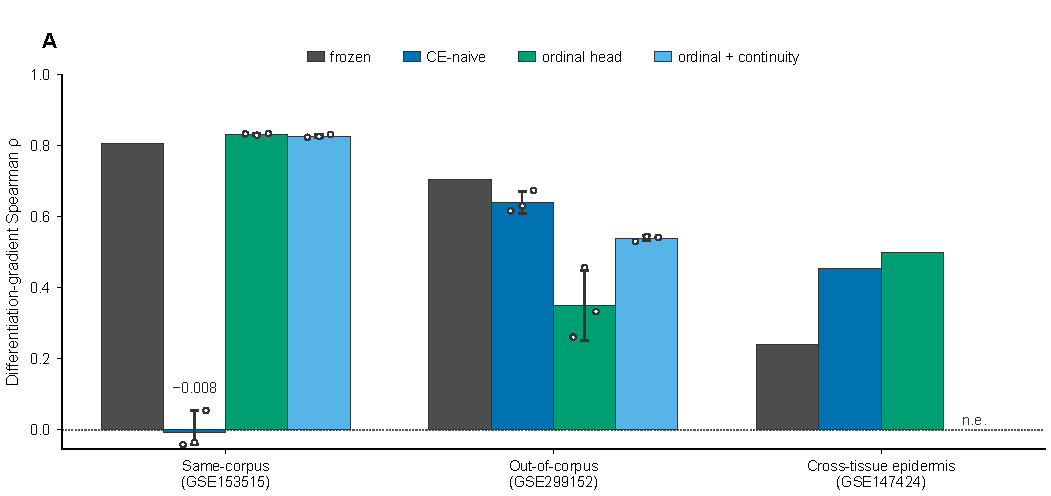
\includegraphics[width=1.0\textwidth]{../../../../figures/paper1/figure5_domain_boundary}
\caption{The collapse depends on the evaluation domain: a three-domain boundary map. Differentiation-gradient Spearman $\rho$ by evaluation domain and arm (frozen, CE-naive, ordinal head, ordinal + continuity). Same-corpus GSE153515 (n = 14{,}775 epithelial cells), out-of-corpus GSE299152 (n = 21{,}374) and cross-tissue epidermis GSE147424 (n = 18{,}355). Same-corpus adapted values are three-seed means whose interval is the full per-seed min--max range (seeds 42, 123, 456), with the individual seeds plotted as open circles; out-of-corpus adapted values are three-seed means $\pm$ 1 sample SD; frozen and cross-tissue adapted arms are single runs with no interval. The same-corpus CE-naive mean ($-0.008$) is labelled at the axis; ordinal + continuity is not evaluated on cross-tissue (n.e.).}\label{fig:domains}
\end{figure}

\begin{figure}[htbp]
\centering
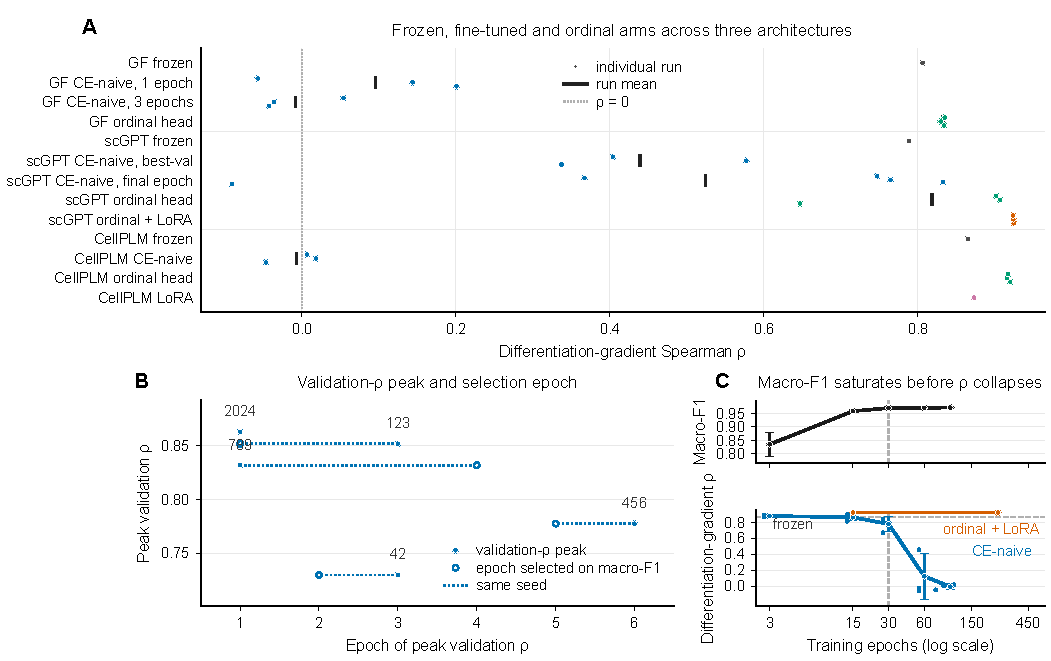
\includegraphics[width=1.0\textwidth]{../../../../figures/paper1/figure6_cross_architecture_spectrum}
\caption{Cross-architecture spectrum of differentiation-gradient collapse. (A) Differentiation-gradient Spearman $\rho$ for Geneformer-V2-104M (GSE153515; n = 14{,}775), scGPT-human (van Zyl; n = 20{,}158) and CellPLM. Individual runs are points, a black tick marks the run mean, and the dotted line marks $\rho = 0$; Geneformer's official-budget row plots seeds 42, 123, 456. Colours: frozen dark grey; CE-naive blue (all CE rows); ordinal head green; LoRA pink-purple; ordinal + LoRA orange-red. Per-seed values: Tables S6--S11. (B) Validation-$\rho$ peaks for scGPT-human (seeds 42, 123, 456, 789, 2024); dotted connector marks the macro-F1 selection epoch. (C) CellPLM dose response, drawn as two stacked panels that share the log-epoch axis: macro-F1 (top; three-seed mean $\pm$ SD) and differentiation-gradient $\rho$ (bottom), for naive cross-entropy and ordinal + LoRA at 15 epochs and convergence; the vertical dashed guide marks the first budget whose mean macro-F1 reaches its plateau (epoch 30), and the horizontal dashed rule is the frozen reference.}\label{fig:spectrum}
\end{figure}

\section*{Discussion}

Classification fine-tuning improved Geneformer annotation, while the differentiation gradient recovered from its embeddings fell to near zero over the same runs and high layer adjacency accuracy persisted alongside this loss. The affected readouts were biologically specific: naive fine-tuning largely flattened the stemness association while partially retaining the differentiation-pole signal. Frozen and ordinal representations recovered declining stemness and increasing differentiation, whereas the proliferative compartment associated with corneal renewal was identified by fixed expression differences, not by axis-dependent gradient retention. The organization of stem and proliferative compartments provides the biological context for these comparisons \cite{cotsarelis1989}. In epidermis, basal-keratin expression supplies a readout of the basal-to-suprabasal transition \cite{fuchs1980}, and adapted arms consistently recovered its basal-off component, while frozen representations emphasized different parts of the transition across datasets. Fine-tuning masking reports that downstream scores obscure pretraining-scale differences \cite{finetuningmasking2026}, whereas paired measurements expose changes in readable differentiation geometry while annotation improves. Classical baselines on the same locked test donor already recovered the axis at correlations of 0.840 to 0.865, so the comparison concerns the readability of an existing gradient rather than the superiority of foundation-model representations.

The direction and location of change depended on the data and model: loss was severe on the same-corpus corneal holdout, smaller on the post-cutoff test, and reversed in epidermal controls. Stronger frozen gradients tended to accompany larger losses, although scGPT-human's weak epidermal gradient was unstable across seeds, and the same-corpus corneal and epidermal sources were both represented in the Geneformer corpus. CellFM offers a gene-level parallel: immune-gene relationships persisted after immune-cell adaptation but disappeared after non-immune-cell adaptation \cite{zeng2025cellfm}. Geneformer lost its gradient under both the official one-epoch budget and the longer main protocol, and in scGPT-human final checkpoints ranged from collapse to retention, while validation selection changed the outcome. In CellPLM the loss appeared only after accuracy had saturated: the three-seed mean fell below 0.2 by sixty epochs, although one of the three seeds retained 0.457, so the timing of the loss, not only its presence, differed between architectures. Head-initialization changes also altered the endpoint with the remaining protocol fixed. Geneformer retained intermediate-layer signal while losing it near the output, and CellPLM showed an early drop at the entry layer, so these depth differences make layer choice relevant to recovering differentiation information from an adapted model. In a frozen Geneformer, circuit-level steering places layer-dependent control of maturation in the same later layers \cite{kendiukhov2026circuits}. That preprint steers a pretrained model, whereas the change measured here arises from adaptation, so the two results are complementary rather than equivalent.

An ordinal head retained the same-corpus Geneformer gradient with observed macro-F1 close to the cross-entropy result. Its stage-order prior targets the progression needed for differentiation analysis, whereas hierarchical cross-entropy uses subtype relationships to improve annotation across studies \cite{hce2026} and EMP-FM supplies process-specific pseudotime supervision for intermediate-state resolution \cite{pan2024}. The stage-order objective retains a gradient already accessible before adaptation. On the scGPT-human same-corpus test, ordinal + LoRA improved gradient retention and macro-F1 over cross-entropy or LoRA alone under the matched longer-budget, best-validation convention, with a narrow seed spread: LoRA represents backbone updates with trainable low-rank increments. The ordinal head arm used a shorter budget and a different checkpoint convention, so the matched comparison concerns the combined recipe. scPEFT measures retention through cell-type confusion after updating \cite{he2026scpeft}, and the gradient adds an endpoint for the organization of differentiation states. The separate ordinal head recipe lost its advantage over cross-entropy on the post-cutoff test (three-seed means), and the combined ordinal + LoRA recipe has been evaluated only on the same-corpus test.

Geometric scores describe information accessible through a particular readout. In protein models, EmmaEmb distinguishes low neighborhood alignment from absence of information recoverable by a nonlinear classifier, and its ProtTucker/ProtT5 comparison also identifies targeted contrastive reorganization with core geometry retained \cite{emmaemb2026}. Intermediate-layer retention in Geneformer and preservation under fixed-frozen-axis projections support a change in accessible ordering and do not require that all differentiation information has disappeared. In that control, the reference direction is fitted once to the frozen model and reused for adapted checkpoints, separating the choice of projection from the embedding update. The stage-rank readout complements the relational measures used in biology-aware benchmarks \cite{wu2025,hou2026}, and scTRAM assesses local neighborhood scrambling and global branch misordering across scales \cite{sctram2025}. A representation can retain a stage ranking while reorganizing branches or local neighborhoods, and rank preservation addresses only one of these properties.

NESS combines agreement with known biology and stability under random initialization to assess embedding reliability \cite{ness2026}. NESS perturbs optimization of a low-dimensional neighbor embedding, whereas our repeated fine-tuning perturbs learned model weights before the differentiation readout is measured. Our PCS-guided evaluation pairs training-seed variation with axis and marker perturbations, donor separation, and corpus-aware tests. Technical and sampling nuisance perturbations probe another source of neighborhood variation \cite{nuisance2026}. Grouped validation addresses dependence between related cells: random splits can distribute clone, patient, or batch relatives across training and evaluation, inflating the apparent number of independent observations \cite{cellleak2026}. Donor-disjoint tests assess between-individual transfer, and post-cutoff tests address pretraining exposure in a new source. For differentiation analysis, representation layers and checkpoints need evaluation against the intended biological readout in an appropriate held-out population.

Three checks follow for practice. First, evaluate an adapted embedding on the biological ordering the downstream analysis needs, not only on held-out labels: in Geneformer, donor-level macro-F1 rose from 0.4421 to 0.6492 while the stage ordering fell from 0.8064 to -0.0082, and layer adjacency moved by only 0.010, about 3\% of the separation between either arm and the permutation null. Second, read intermediate layers before concluding that the information is gone, because the loss sat in Geneformer's upper layers rather than throughout the model. Third, treat seed and checkpoint selection as part of the result, because one scGPT-human configuration produced both collapse and retention. Stage-ordered supervision retained the gradient in our same-corpus tests, but the separate Geneformer ordinal head recipe lost its advantage on the post-cutoff test (three-seed means), and the combined ordinal + LoRA recipe has not been evaluated out of corpus.

\section*{Limitations of the study}

\textbf{Pretraining exposure.} Source-publication matches establish corpus provenance more directly than inclusion of individual cells or donors, and donor exposure in the Geneformer holdout is conservatively presumed. Pretraining exposure is therefore incompletely observable, which limits interpretation of the frozen gradient as generalization.

\textbf{Coverage.} The primary holdout has two donors, the post-cutoff corneal test has three, and the scGPT-human comparison has one test donor. Cell-level confidence intervals in that arm therefore quantify uncertainty conditional on the sampled individual. Seed coverage is uneven, with several CellPLM and supplementary configurations represented by fewer runs. Budgets and checkpoint conventions also differ across model families and some recipes, so matched comparisons apply to the specified subsets, including the longer-budget scGPT-human LoRA comparison, but not to every arm.

\textbf{Annotation-informed axis.} The three- and four-stage references summarize differentiation order without reconstructing a complete continuous or branching trajectory, and their different resolutions constrain direct cross-dataset comparisons. The projection axis is fitted to labelled centroids, and annotation and program analyses share some markers, introducing dependence between the biological reference and its molecular interpretation. Alternative marker panels and fixed-axis controls address particular analysis choices, while the fitted readout remains dependent on the available annotations.

\textbf{Unvalidated out of corpus.} The combined ordinal + LoRA recipe was evaluated only on the same-corpus scGPT test, and the out-of-corpus evidence rests on the separate Geneformer ordinal head recipe. The association between frozen-axis strength and adaptation outcome was observed across datasets whose tissue composition, sampling, and adaptation context also differ, and axis strength itself was not independently manipulated.

\section*{Methods}

\subsection*{1. Data sources and preprocessing}

\textbf{Training atlas.} Training and internal-test data came from the Single cell atlas of the human ocular surface collection in CELLxGENE Discover (collection identifier \texttt{0f7d022a-\allowbreak 46c7-\allowbreak 4e64-\allowbreak be4c-\allowbreak e34adbb78089}; dataset identifier \texttt{8ef06ea4-\allowbreak 8d0f-\allowbreak 4303-\allowbreak a652-\allowbreak 7d4604402b1f}). The downloaded dataset version is described by its file identifier, download size, recorded MD5, schema version, and publication date in Supplementary Methods. This pre-publication consortium resource, produced by CZI Cell Science and the Human Cell Atlas Eye Network, had no journal publication or DOI and was cited as a CELLxGENE collection \cite{chen2026cellxgene}. It aggregated ten studies of corneal, limbal, scleral, and fetal ocular surface tissues \cite{li2021oculsurf,li2021iovs,maiti2022,collin2021,dou2021,catala2021,gautam2021}. The combined AnnData object contained 120,000 cells, with 20 curated and 31 author-assigned cell-type labels.

Author labels were mapped to five differentiation layers: limbal stem cells (LSC, including LPC and fetal epithelial progenitors; index 0), transient-amplifying cells (TAC, limbal epithelium; index 1), basal cells (Epi-PMC; index 2), wing cells (Epi-TDC/PMC; index 3), and squamous cells (Epi-TDC/unknown epithelium; index 4). Non-epithelial populations, including immune, endothelial, stromal, conjunctival, and melanocyte populations, received index $-$1 (\texttt{NON\_\allowbreak LAYER}) and were excluded from ordinal measurements. For the external four-class task, wing and squamous cells were merged into a differentiated class, yielding LSC, TAC, basal, and differentiated stages.

\textbf{External tests.} GSE153515, a 10x Genomics dataset of normal human limbal basal epithelium \cite{li2021oculsurf,li2021iovs}, contained 17,587 cells from two donors (GSM4646295 and GSM4646296) and 32,738 input features. GSE299152, an ocular surface glycocalyx atlas \cite{gse299152}, contained 26,628 human cells from three donors and 36,601 input features; mouse cells were not used. These datasets provided the same-corpus and post-cutoff out-of-corpus tests, respectively, for Geneformer. Corpus status is distinguished from separation from the adaptation atlas in Section 12; the programmatic cross-checks between the external tests and the adaptation-atlas studies are reported in Supplementary Methods.

\subsection*{2. Fair donor-disjoint splitting protocol}

The adaptation atlas was split by donor before model fitting. Deterministic assignment with seed 42 allocated 49 donors (99,606 cells) to training and 25 donors (20,394 cells) to internal testing, with no donor overlap. Within the training partition, a deterministic stratified 80/20 split (seed 42) gave 79{,}684 fitting cells and 19{,}922 internal-validation cells; every adapted arm batches the 79{,}684 fitting cells, which is why the three-epoch Geneformer arms run 7{,}473 optimizer steps at an effective batch of 32. Both partitions represented all 20 curated and all 31 author-assigned labels. A locked manifest recorded donor lists, cell counts, label distributions, and SHA-256 checksums of the train and test AnnData files; no cells were reassigned afterward. The manifest is included in the released artifact bundle (Data and code availability). Donor grouping addresses dependence between cells from the same individual that a cell-level random split would not remove \cite{cellleak2026}.

\subsection*{3. External test annotation pipeline}

GSE153515 lacked observation-level annotation metadata. Its labels were constructed with \texttt{scripts/\allowbreak protocol\_\allowbreak 15\_\allowbreak annotate\_\allowbreak gse153515.py} before model evaluation, using parameters locked in a configuration file (Supplementary Methods). Eight curated marker sets covered LSC, TAC, basal, differentiated, conjunctival, melanocyte, immune, and stromal identities and were scored on the full 32,738-feature matrix (Figure S8).

Quality control applied minimum-gene-count and maximum-mitochondrial-fraction filters specified in the locked configuration. It retained 15,827 of 17,587 cells (90.0\%) and 10,605 genes (Figure S4). Highly variable gene selection, log-normalization, scaling, and PCA preceded Harmony correction \cite{korsunsky2019} and Leiden clustering (parameters in Supplementary Methods; Figure S12). Cluster-specific differentially expressed genes were identified by the Wilcoxon rank-sum test. Marker enrichment among the top 200 genes was scored as

\[
E = \frac{n_{\mathrm{in\ top\ 200}}}{n_{\mathrm{total}}}
\left(1-\frac{\mathrm{mean\ rank}}{200}\right).
\]

Clusters below the epithelial enrichment threshold of 0.3 were assigned \texttt{NON\_\allowbreak LAYER}. Four-class harmonization retained 14,775 epithelial cells: 3,423 LSC, 171 TAC, 6,698 basal, and 4,483 differentiated cells. Non-epithelial cells were excluded from external epithelial evaluation.

GSE299152 used the corresponding pipeline and configuration (\texttt{scripts/\allowbreak protocol\_\allowbreak 15b\_\allowbreak annotate\_\allowbreak gse299152.py}; configuration file in Supplementary Methods); its two recorded deviations and its flagged low-confidence clusters are described there. Quality control retained 23,970 of 26,628 cells (90.0\%) and 11,274 genes. Harmonization yielded 15,921 LSC, 1,099 basal, and 4,354 differentiated cells, totaling 21,374 epithelial cells; 2,596 non-epithelial cells were excluded. No TAC class was assigned because proliferation markers occurred in fewer than 0.6\% of cells.

\subsection*{4. Model architectures}

The Geneformer comparison included two non-adapted references and five adapted configurations differing in supervision, loss-contributing cells, label set, optimizer-step budget, and head design.

\textbf{Arm 1: HVG/PCA with a linear classifier.} Highly variable genes were selected from the training partition. Expression was log-normalized and scaled, PCA was fitted, and a linear classifier was trained on the resulting components.

\textbf{Arm 2: frozen Geneformer with a linear probe.} Geneformer-V2-104M was loaded from the Hugging Face model hub (snapshot commit and recorded weight hash in Supplementary Methods). The pretrained model used a 12-layer BertForMaskedLM encoder (attention heads, hidden dimension, and vocabulary size in Supplementary Methods). Its Genecorpus-104M pretraining resource comprised approximately 104 million cells from 2,903 datasets \cite{theodoris2023,chen2026natcompsci}. Transformer weights were frozen, and a linear classifier was fitted to the [CLS] representations.

\textbf{Arm 3: naive Geneformer fine-tuning.} The full model was fine-tuned with cross-entropy over the 31 author-assigned labels, with no continuity term ($\lambda=0$). Predictions were merged into the four epithelial classes for external evaluation. Non-epithelial author labels contributed to the training classification loss.

\textbf{Arm 4: ordinal head Geneformer.} The full model was fine-tuned using unconditional cumulative-threshold binary cross-entropy with $\lambda=0$. Only epithelial targets contributed to this loss. Non-epithelial cells remained in the input batches but were masked out of ordinal supervision.

\textbf{Arm 5: ordinal + continuity Geneformer.} This configuration combined the same ordinal loss with the continuity term at $\lambda=0.5$. A centroid computation supporting variable-length inputs allowed the continuity objective to execute (Section 5).

\textbf{Arm 6: epithelial-only four-class cross-entropy (2{,}616 steps).} Same model, split, optimizer settings and three seeds as Arm 3, with two changes: the training partition was restricted to the 27{,}878 epithelial cells, and the classification head predicted the four stage classes directly (LSC, TAC, basal and differentiated, with wing and squamous merged as in the external evaluation) rather than the 31 author-assigned classes. Three epochs over the epithelial subset give 2{,}616 optimizer steps.

\textbf{Arm 7: epithelial-masked four-class cross-entropy (7{,}473 steps).} The same four stage labels and the same supervised cells as Arm 6, but the 51{,}806 non-epithelial training cells were retained in the batches and excluded from the loss, so the arm runs the full 7{,}473 optimizer steps used by Arms 3--5. No auxiliary loss term was active ($\lambda = 0$). Read with Arm 6, this pair separates the optimizer-step budget from the label set.

Arms 3--5 were trained for three epochs with seeds 42, 123, and 456. Per-seed coverage is given in Table S1; the training hyperparameters are listed in Supplementary Methods (Figure S5).

\subsection*{5. Ordinal head formulation}

Ordinal supervision encoded stage order through unconditional cumulative binary targets. For $K=4$ corneal stages, three logits $f_{ik}$ per cell were trained against $t_{ik}=\mathbf 1(y_i\ge k)$, $k=1,\ldots,K-1$. With $N_E$ epithelial cells in a batch, the loss was

\[
\mathcal L_{\mathrm{ord}}=
\frac{1}{N_E(K-1)}
\sum_{i\in E}\sum_{k=1}^{K-1}
\operatorname{BCEWithLogits}(f_{ik},t_{ik}).
\]

Reduction was a mean across valid cells and thresholds. All valid epithelial cells contributed to every threshold, without conditional training subsets or a cumulative-product transformation. This \textbf{unconditional cumulative-threshold ordinal head} differs from standard conditional CORN \cite{shi2023corn,onc2025}. The scGPT-human and CellPLM ordinal implementations likewise used unconditional threshold BCE with mean reduction and sigmoid threshold-count decoding; their three-stage task required two thresholds.

For Geneformer, logits were produced by the classifier from the dropout-transformed pooled BERT output. Geometric evaluation used the position-0 final hidden state. At inference, $p_k=\sigma(f_k)$ and the hard stage prediction was $\hat y=\sum_k\mathbf 1(p_k\ge0.5)$. The independent outputs were unconstrained. Monotonicity was evaluated afterward by checking $p_1\ge p_2\ge\cdots\ge p_{K-1}$ within each cell and comparing with a within-cell permutation null (Figure S10).

For Geneformer probability-based evaluation, adjacent probability differences were clipped at zero and each row renormalized to sum to one; macro-F1 used threshold-count hard predictions, whereas ECE used the maximum probability and argmax class of this repaired distribution (construction and Figure S2 in Supplementary Methods). These are different decoding rules and need not yield the same class; ECE therefore does not automatically calibrate the exact decision rule used for macro-F1.

The ordinal head arm used this loss alone. The ordinal + continuity arm added a continuity term at weight 0.5. Training centroids were recomputed before each epoch by a callback for variable-length inputs (callback name in Supplementary Methods). The continuity calculation used the five-layer training map; the ordinal loss used its four-stage harmonization.

\subsection*{6. Evaluation metrics}

The primary external evaluations used the locked Tier-B pipeline (\texttt{corneal\_\allowbreak fm/\allowbreak evaluation.py}). Cell identities and reference stage labels were held fixed across the arms being compared.

\textbf{Classification.} The primary endpoint was the arithmetic mean of donor-specific macro-F1 scores over the four specified epithelial classes. Per-class precision, recall, F1, and support were also reported. Nonparametric 95\% confidence intervals resampled donor identifiers with replacement, averaging their precomputed macro-F1 scores in each of 1,000 draws (seed 42); limits were the 2.5th and 97.5th percentiles. On the two-donor GSE153515 test this quantifies variation over the two observed donors, not broad population-level uncertainty. Adapted-arm table summaries averaged the per-seed point estimates and the respective per-seed interval bounds. These averaged bounds are not a joint donor-and-training-seed confidence interval. Reference arms were single runs.

\textbf{Differentiation-gradient correlation.} The metric measured Spearman correlation between an embedding-derived projection and the specified stage rank, excluding \texttt{NON\_\allowbreak LAYER} cells. For each evaluated checkpoint, centroids were computed from the \textbf{evaluation cells grouped by their reference stage labels}. The first right singular vector of the centered centroid matrix defined the projection axis. Its sign was oriented from the first to the last present stage; projecting each cell onto this axis yielded the axis pseudotime. The resulting correlation is an annotation-informed geometric readout, not label-free trajectory inference or prediction of unseen stage labels. Marker expression was not an input to this centroid calculation, although marker-derived annotations supplied the stage groups. Where specified for scGPT-human, embeddings were L2-normalized; raw-embedding measurements were retained separately.

\textbf{Other endpoints.} Layer adjacency accuracy (LAA) was the fraction of cells whose nearest other cell in Euclidean embedding space had an identical or adjacent stage. Expected calibration error (ECE) was the frequency-weighted absolute difference between accuracy and confidence across ten probability bins, with confidence 1 included in the last bin (Figure S1). For ordinal Geneformer, its probability-based argmax rule is distinguished from threshold-count classification in Section 5.

\textbf{Layer-resolved measurement.} The embedding output (L0) and all 12 Geneformer transformer hidden states were collected for the 14,775 GSE153515 epithelial cells, and at each depth the position-0 [CLS] representation was used to recompute the centroid-axis metric (collection, consistency-gate, bootstrap, and randomized-head details in Supplementary Methods; Figure 2).

\textbf{Trajectory and rare-class diagnostics.} Diffusion pseudotime and a rare-TAC-exclusion sensitivity analysis were computed from the external embeddings and correlated with the reference layer-order pseudotime (settings in Supplementary Methods; Figures S9 and S11).

\textbf{Marker-program readouts.} Program scores were fixed across models: genes were log1p-transformed and standardized, and each program score was the unweighted mean of its genes. The stemness score comprised \textbf{TP63, KRT15, KRT19, NFIB, and CDH3}; corneal differentiation used KRT12 and KRT3; cycling used PCNA, MCM2, MKI67, and TOP2A. Each expression score was correlated with model-specific axis pseudotime; the epidermal gene lists, the interval and null settings, and the overlap between program genes and the annotation marker sets are given in Supplementary Methods.

\subsection*{7. Axis definition revision (protocol deviation)}

Auxiliary-objective training initially used a marker-score reference axis. Seed-42 evaluation identified a direction mismatch with the centroid-PCA evaluation definition (cosine alignment 0.470). On 2026-08-10, an approved protocol deviation replaced the training reference with a centroid-PCA axis fitted across epithelial \textbf{training} cells (\texttt{corneal\_\allowbreak fm/\allowbreak axis\_\allowbreak ref.py}; implementation mode, cache schema, and changelog identifier in Supplementary Methods). The revised axis definition was used for cross-tissue evaluation. The training reference and checkpoint-specific test axis shared a construction rule; they were not the same fitted vector or the same input cells.

Sensitivity analyses on the van Zyl test donor varied the SVD definition, marker panels, and ranks; the tested variants and the SVD validation of the centroid-axis implementation are listed in Supplementary Methods. A separate fixed-frozen-axis control fitted a direction once from the frozen model's labeled test-donor centroids and reused it to project adapted embeddings. This held projection selection fixed across checkpoints, but did not remove the frozen reference axis's dependence on the annotated test population.

\subsection*{8. Cross-architecture frozen probes (scGPT-human, scFoundation, UCE)}

\textbf{scGPT-human.} Frozen representations used \texttt{perturblab/\allowbreak scgpt-\allowbreak human} (12-layer Transformer, hidden dimension 512, 51.86M parameters; software version and commit in Supplementary Methods). Continuous log1p inputs were tokenized with its gene vocabulary, retaining CLS first (vocabulary size, sequence length, and tokenizer flags in Supplementary Methods). The final CLS representation supplied the embedding. The centroid-derived stage-rank metric was the same geometric definition used above, not a direct marker-expression correlation. The frozen probes were self-probes of separability within an evaluation dataset, not donor-disjoint transfer performance (probe construction in Supplementary Methods).

\textbf{scFoundation.} The 01B-resolution checkpoint was obtained from the \texttt{genbio-\allowbreak ai/\allowbreak scFoundation} mirror; its recorded SHA-256 prefix, inference entry point and arguments, and vocabulary-alignment counts are given in Supplementary Methods. Its xTrimoGene encoder--decoder had 119.25M parameters \cite{scfoundation2024}. The concatenated cell embedding (dimension in Supplementary Methods) pooled last-layer, second-to-last-layer, max-pooled, and mean-pooled representations. The pretraining corpus exceeded 50 million human cells but was not publicly enumerated. Membership of either external source was therefore unknown, not demonstrated to be out-of-corpus.

\textbf{UCE.} Official inference used the 33-layer checkpoint (checkpoint filename, Figshare DOI, and recorded SHA-256 in Supplementary Methods) \cite{rosen2026uce}; inference used human species and expression-weighted gene sampling, producing a CLS embedding followed by L2 normalization (embedding dimension, entry point, sampling, and padding settings in Supplementary Methods). Each dataset was embedded with seeds 42, 123, and 456 because gene sampling was stochastic. Correlations and probe macro-F1 were averaged across these inference repeats (Table S4); these repeats were not independent fine-tuning runs. UCE used census release 2023-04-25. GSE153515 was absent from the closest queryable release, 2023-05-15, and GSE299152 postdated the corpus; their out-of-corpus designation for UCE was consequently inferential.

\subsection*{9. Cross-architecture fine-tuning protocols (van Zyl same-corpus arm and official-budget controls)}

\textbf{Training conventions.} The main Geneformer comparison used three epochs. Additional controls followed the one-epoch Geneformer convention \cite{theodoris2023} and the 15-epoch, best-validation scGPT convention \cite{cui2024scgpt} under a preregistered amendment (PREREG \S9).

\textbf{van Zyl same-corpus dataset.} The van Zyl limbal and central cornea atlas \cite{vanzyl2022} was the corneal source in scGPT-human's census 2023-05-15 pretraining release. A preregistered exclusion removed 13,584 ciliary-muscle cells in Leiden cluster 0, leaving 62,640 epithelial cells (PREREG \S7). The stage reference had three tiers, LSC $\rightarrow$ basal $\rightarrow$ differentiated, because the locked gene filter removed all six cycling markers needed to assign TAC. The largest epithelial donor, Hu0216 (20,158 cells), was locked as the test donor; four other donors supplied 42,482 cells (PREREG \S8).

The preregistered frozen-axis gate G1, the revised training-adequacy gate G0 with its historical reference, and the frozen-probe caveats are specified in Supplementary Methods. Frozen geometry and permutation-null calculations used the three-tier centroid-axis definition.

\textbf{scGPT arms and checkpoints.} Naive cross-entropy used 30 author-assigned labels under the shared scGPT training hyperparameters (Supplementary Methods). The three-epoch ordinal head configuration used all 42,482 training-donor cells and a final checkpoint. The 15-epoch protocol reserved 4,247 cells (10\%) for validation by stratified donor-by-layer sampling with seed 42, leaving 38,235 cells for fitting; the validation manifest was SHA-256-locked before training, and Hu0216 did not enter training or validation. This split was shared by the longer-budget cross-entropy, LoRA-only, and ordinal + LoRA comparisons, whose checkpoints were selected by validation macro-F1. Test-donor confidence intervals used cell-level resampling because only one test donor was available. Seeds 42, 123, and 456 defined the best-validation recipe summaries; the final-epoch cross-entropy sensitivity summary used seeds 42, 123, 456, 789, and 2024 and was kept separate from the three-run comparison. The combined ordinal + LoRA configuration used the unconditional ordinal head from Section 5 and LoRA on query, key, and value projections in all 12 scGPT-human transformer layers ($r=8$, $\alpha=16$), with 38,235 fitting cells, 4,247 validation cells, 15 epochs, and selection by validation macro-F1, run with seeds 42, 123, and 456 and Hu0216 held out. Ordinal+LoRA was evaluated on the same-corpus van Zyl test; the post-cutoff ordinal head evaluation used a separate recipe.

\textbf{Geneformer official-budget control.} Naive cross-entropy training was repeated for one epoch with the main Geneformer split, hyperparameters, and locked GSE153515 test. Seeds were 42, 123, 456, 789, 2024, and 31415, distinct from the three-seed main three-epoch comparison.

\textbf{CellPLM.} The third family was CellPLM v1.0.0, an 85M-parameter Flowformer encoder with a latent VAE representation \cite{wen2024cellplm}. Main van Zyl cross-entropy and unconditional ordinal configurations each used seeds 42, 123, and 456, with 38,233 fitting cells, 4,249 validation cells, and the 20,158-cell Hu0216 test. They used the official \texttt{CellTypeAnnotationPipeline}, with a three-class cross-entropy head or two ordinal threshold outputs on the three-stage axis, and the official pipeline settings; checkpoints were selected by validation F1 and saved as \texttt{model\_\allowbreak best\_\allowbreak valid.pt} (hyperparameters, epoch cap, stopping parameters, and HVG panel size in Supplementary Methods). Training lasted 78/123/129 epochs for the ordinal arm and 83/118/97 epochs for the cross-entropy arm (seeds 42/123/456), under the 2,000-epoch cap; these were not fixed three-epoch runs. Test evaluation used 1,000 cell-bootstrap replicates and 100 label-shuffle replicates, and three-seed recipe summaries used sample SD. The CellPLM LoRA and layer-resolved evaluations were single-seed analyses (seed 42), with adapter and layer settings in Supplementary Methods; the supplementary two-seed replication is specified in Section 11.

\subsection*{10. Head-init basin selection}

The scGPT-human naive configuration was repeated with the seed-42 backbone and three alternative head initializations: classifier-weight scales 0.01 and 1.0, and head seed 999. Backbone weights, data, objective, and training budget were otherwise held fixed. Both final and best-validation checkpoints were evaluated on Hu0216. These were training-time initialization perturbations, distinct from the inference-only randomized-head diagnostic in Section 6. Variants are compared descriptively with the default endpoint.

\subsection*{11. Supplementary evaluation protocols}

The GSE147424 epidermal control, the Hu0220 corneal leave-one-donor test, the GSE186433 and GSE155683 corneal tests, and the CellPLM two-seed consistency replication followed the same locked adaptation protocols; their cell counts, partitions, input settings, replication details, and the source status of the two corneal tests are given in Supplementary Methods.

\subsection*{12. Provenance and contamination audit}

Separation of the adaptation atlas from a test dataset was assessed independently of that test source's possible pretraining exposure; the download, retrieval, checksum, and manifest version-lock record is given in Supplementary Methods.

A source-publication audit of the Geneformer-V2 Genecorpus-104M supplementary source table permitted the corpus assignment of each dataset (manifest counts, table location, matched DOIs, cell counts, and public dates in Supplementary Methods). GSE153515 was treated as same-corpus rather than a pretraining-naive test. GSE299152 \cite{gse299152} postdated assembly and had no matching DOI, providing the post-cutoff out-of-corpus test.

The GSE147424 source \cite{he2020epidermis} and GSE202352 \cite{wiedemann2023} each matched a skin row and were thus in-corpus cross-tissue controls for Geneformer; corpus membership was not treated as a measurement of frozen-axis strength. For scGPT-human, census release 2023-05-15, GSE153515 was absent from the curation catalog and the census manifest while GSE299152 postdated it, so the two external sources were designated out-of-corpus \cite{cui2024scgpt}. Two adaptation-atlas studies matched corpus DOIs; these source-level matches were not donor-level exposure measurements (study names and cell counts in Supplementary Methods).

\textbf{Exposure limits.} The Geneformer source table recorded publication DOI, filtered cell count, and organ, not donor or accession identities; released shards contained rank-encoded expression, so direct matching of individual test donors was unavailable. We conservatively presumed exposure for the GSE153515 donors rather than claiming a leakage-free frozen baseline, and did not claim to prove that every source donor was ingested. The paired post-cutoff test addressed a different exposure regime; it did not retroactively remove pretraining exposure from the same-corpus result.

A bounded cell-fingerprint check, motivated by scContam \cite{sccontam2026}, sampled a fraction of the source corpus and found no hits among the GSE153515 cells, with full positive-control recall and no negative-control false positives (sampled fingerprint count and fraction, MinHash parameters, and the observed maximum Jaccard in Supplementary Methods). This check validated the pipeline within the sampled material; its negative result did not exclude exposure. The DOI audit remained the primary provenance evidence.

\subsection*{13. Software, reproducibility, and statistical analysis plan}

The main analysis environment used Python 3.12, Scanpy \cite{wolf2018scanpy}, harmonypy \cite{korsunsky2019,harmonypy}, Hugging Face Transformers \cite{wolf2020transformers}, PyTorch \cite{paszke2019}, and scikit-learn \cite{pedregosa2011}; model-specific versions and inference settings, and the custom modules and analysis entry points, are listed in Supplementary Methods.

Statistical summaries distinguished donor resampling, cell resampling conditional on the observed donor(s), and variation across training seeds. The primary Geneformer external family comprised 26 tests with Benjamini--Hochberg FDR control at $q=0.05$. For gradient correlations, the adjusted q values tested positive association, not differences between adaptation arms. Arm contrasts were quantified by a paired donor-stratified cell bootstrap with 2{,}000 replicates per seed: cells were resampled with replacement within each external-test donor, the same resampled cells were used for both arms, and the stage-centroid axis was refit on the resampled cells in every replicate rather than held at its full-sample value, a choice that widens the interval roughly fourfold. Across the three training seeds the per-seed replicate arrays were concatenated (three seeds $\times$ 2{,}000 replicates) and each quoted interval is the 2.5th to 97.5th percentile of that pooled distribution. Layer adjacency accuracy was referred to a label-permutation null in which stage labels were reshuffled across cells (2{,}000 permutations) with the class counts and the nearest-neighbour graph held fixed; the null mean was 0.642 for all arms. The separate cross-model correction family had fixed membership and comprised 21 evaluated tests, with six further entries pending at freeze time and the later-completed CellPLM and combination runs held outside it (family membership and pending entries in Supplementary Methods). Reporting conventions for permutation statistics, interval types, and interval overlap are given in Supplementary Methods.

\textbf{Operational terminology.} The preregistered van Zyl frozen-axis gate G1 required both $\rho\ge0.5$ and label-shuffle $z\ge3$. Falling below its correlation component was used as a descriptive threshold in reports of gradient loss; it was not a universal biological threshold, and weak-axis cross-domain frozen references were not claimed to pass G1. The historical severity convention labeled correlations near zero, using $\rho<0.2$, as catastrophic and intermediate reductions as moderate or partial. Because this signed cutoff also includes negative correlations, reversed orderings were reported with their actual signed values rather than silently equated with noise. Retention relative to a frozen reference was described within the relevant seed and checkpoint stratum, not inferred from interval overlap. These labels summarize the specified stage-rank readout; they do not establish loss of all differentiation information or reconstruction of a complete continuous or branching trajectory.

\section*{RESOURCE AVAILABILITY}

\subsection*{Lead Contact}

Further information and requests for resources should be directed to and will be fulfilled by the lead contact, Qi Dai (dq@mail.eye.ac.cn).

\subsection*{Materials Availability}

This study did not generate new unique reagents or biological materials; all data are public (below).

\subsection*{Data and Code Availability}

\begin{itemize}
\item \textbf{Training data.} CELLxGENE Discover collection 0f7d022a-46c7-4e64-be4c-e34adbb78089 (Single cell atlas of the human ocular surface; Human Ocular Surface Atlas), current dataset-version of dataset 8ef06ea4-8d0f-4303-a652-7d4604402b1f, distributed as file 30127f02-d0b9-4b56-bf4c-e5b77e4989bd.h5ad; MD5 39f098367af95bc3e1ee92528ceb251e.
\item \textbf{External test data.} GEO GSE153515 \cite{li2021oculsurf}; 17{,}587 cells from two donors (GSM4646295, GSM4646296). GEO GSE299152 \cite{gse299152}; 21{,}374 epithelial cells from three donors after QC. Cross-tissue: GEO GSE147424 \cite{he2020epidermis}.
\item \textbf{Cross-architecture probes.} scGPT-human checkpoint (perturblab/scgpt-human; scgpt 0.2.5, git commit cebd6fae); CellPLM v1.0.0; scFoundation 01B-resolution checkpoint (genbio-ai/scFoundation Hugging Face mirror); UCE 33-layer checkpoint (Figshare 10.6084/m9.figshare.24320806); frozen-probe diagnostics in results/scgpt\_repro/frozen\_diag/, results/scfoundation\_repro/frozen\_diag/, and results/uce\_repro/frozen\_diag/.
\item \textbf{Model.} Geneformer-V2-104M, Hugging Face model hub (ctheodoris/Geneformer; snapshot commit 04c2b2e84da7c0f385c3f9ad8f3ec24bab6650e5).
\item \textbf{Code.} Analysis code, evaluation scripts, and aggregated result files are maintained at \url{https://github.com/Xu-Kunk/Cornea-Ai}. Editors and reviewers can obtain access on request, and the repository will be made public with a DOI-minting deposit before publication.
\item \textbf{Evaluation scripts.} All evaluation, baseline, layer-wise, trajectory and statistical scripts are held in \texttt{scripts/\allowbreak}; the entry point used for each analysis is named in the corresponding Methods subsection.
\item \textbf{Results.} Aggregated result files are held under \texttt{results/\allowbreak}: the main protocol in \texttt{results/\allowbreak paper1\_\allowbreak tier\_\allowbreak b\_\allowbreak eval/\allowbreak *.json}, and the cross-architecture arms and statistical controls under \texttt{results/\allowbreak paper1\_\allowbreak vanzyl/\allowbreak}, including the \texttt{corn\_\allowbreak lora/\allowbreak}, \texttt{cellplm\_\allowbreak layerwise/\allowbreak}, \texttt{head\_\allowbreak init/\allowbreak}, \texttt{sensitivity/\allowbreak}, \texttt{fdr/\allowbreak}, \texttt{svd\_\allowbreak validation/\allowbreak}, \texttt{cross\_\allowbreak tissue/\allowbreak}, \texttt{loo/\allowbreak}, \texttt{cornea2/\allowbreak}, \texttt{cellplm\_\allowbreak consistency/\allowbreak} and \texttt{claim\_\allowbreak audit/\allowbreak} subdirectories.
\item \textbf{Reproducibility.} All experiments are reproducible with fixed random seeds (42, 123, 456), locked configuration files, and SHA-256-locked fair-split manifests.
\item \textbf{Additional information.} Any additional information required to reanalyze the data reported in this paper is available from the lead contact upon request.
\end{itemize}

\section*{ACKNOWLEDGMENTS}

We thank the generators of the public datasets used in this study, in particular the Human Ocular Surface Atlas team (van Zyl et al.) and the authors of GSE153515, GSE299152, and GSE147424, for making single-cell data openly available. This work was supported by the National Natural Science Foundation of China (82571251) and the Medical and Health Science Program of Zhejiang Province (WKJ-ZJ-26067).

\section*{AUTHOR CONTRIBUTIONS}

\textbf{K.X.:} conceptualization, methodology, software, investigation, formal analysis, data curation, visualization, writing -- original draft. \textbf{C.W.:} investigation, validation, writing -- review \& editing. \textbf{F.L.:} methodology, supervision, resources. \textbf{X.C.:} investigation, data curation. \textbf{X.W.:} investigation, data curation. \textbf{Y.Z.:} investigation, data curation. \textbf{T.P.:} investigation, validation. \textbf{J.T.:} investigation, visualization. \textbf{H.C.:} resources, supervision. \textbf{P.G.:} resources, supervision. \textbf{Q.D.:} supervision, project administration, writing -- review \& editing.

\section*{DECLARATION OF INTERESTS}

The authors declare no competing interests.

\section*{DECLARATION OF GENERATIVE AI AND AI-ASSISTED TECHNOLOGIES IN THE WRITING PROCESS}

During the preparation of this work, the authors used DeepSeek-V4 series models (DeepSeek), served locally, for language polishing and code development. No scientific data, results, or images were generated by AI. After using these tools, the authors reviewed and edited all content and take full responsibility for the content of the publication.

\section*{SUPPLEMENTAL INFORMATION INDEX}

\begin{description}
  \item Figures S1--S13 and their legends in a PDF
  \item Table S1. Related to Table 1: Primary external-test metrics (per-seed, per-donor, per-class)
  \item Table S2. Related to Table 1: Label-set and step-budget controls
  \item Table S3. Related to Figure 2: Layer-resolved differentiation-gradient Spearman $\rho$ (external test, n = 14,775 cells)
  \item Table S4. Related to Table 1: Frozen-representation probes across single-cell foundation models
  \item Table S5. Related to Methods: Training-atlas composition and provenance record
  \item Table S6. Related to Figure 6: scGPT-human same-corpus arms --- per-seed test-donor metrics across budgets
  \item Table S7. Related to Figure 6: scGPT-human convergence checkpoints (van Zyl, test donor Hu0216)
  \item Table S8. Related to Figure 6: Geneformer official-budget control
  \item Table S9. Related to Figure 6: CellPLM arms
  \item Table S10. Related to Table S12: Classical baselines
  \item Table S11. Related to Figure 6: CellPLM training-budget dose response
  \item Table S12. Related to Figure 6: Geometry-preserving recipes on the scGPT-human van Zyl same-corpus test donor
  \item Data S1. Layer-resolved differentiation-gradient $\rho$ (raw values)
  \item Data S2. Per-cell predictions and embeddings
  \item Data S3. Locked fair-split manifest and SHA-256 checksums
  \item Supplementary Methods: configuration, provenance and software details
\end{description}

\newpage


\bibliography{paper1}

\end{document}
